\documentclass[12pt]{article}
\usepackage{geometry}                % See geometry.pdf to learn the layout options. There are lots.
\geometry{letterpaper}                   % ... or a4paper or a5paper or ... 
%\geometry{landscape}                % Activate for for rotated page geometry
\usepackage[parfill]{parskip}    % Activate to begin paragraphs with an empty line rather than an indent
\usepackage{daves,fancyhdr,natbib,graphicx,dcolumn,amsmath,lastpage,xurl}
\usepackage{amsmath,amssymb,epstopdf,longtable}
\usepackage[final]{pdfpages}
\DeclareGraphicsRule{.tif}{png}{.png}{`convert #1 `dirname #1`/`basename #1 .tif`.png}
\pagestyle{fancy}
\lhead{CE 3354 -- Engineering Hydrology}
\rhead{FALL 2024}
\lfoot{ES1}
\cfoot{}
\rfoot{Page \thepage\ of \pageref{LastPage}}
\renewcommand\headrulewidth{0pt}



\begin{document}
\begin{center}
{\textbf{{ CE 3354 Engineering Hydrology} \\ {Exercise Set 1}}}
\end{center}

\section*{\small{Exercises}}
\begin{enumerate}\item Using the internet, textbook(s), and the on-line reading collection define the following (in a sentance or two); please cite your references (URL is sufficient): 
 \begin{enumerate}
 \item Alluvium 
 \item Bankfull Discharge
 \item Best Management Practice
 \item Drainage Divide 
 \item Evaporation 
 \item Evapotranspiration 
 \item Precipitation 
 \item Flow Duration Curve
 \item Flood Frequency Curve
 \item Watershed 
 \item Catchment
 \end{enumerate}
 
\textbf{Solution(s)}

 \begin{enumerate}
 \item \textbf{Alluvium} (from Latin alluvius, from alluere 'to wash against') is loose clay, silt, sand, or gravel that has been deposited by running water in a stream bed, on a floodplain, in an alluvial fan or beach, or in similar settings 
 \url{https://en.wikipedia.org/wiki/Alluvium}
 \item \textbf{Bankfull Discharge} is the maximum discharge that the channel can convey without overflowing onto the floodplain. 
 \url{http://www.extranet.vdot.state.va.us/locdes/hydraulic_design/nchrp_rpt544/content/html/WorksCited/Copeland_2001.pdf}
 \item \textbf{Stormwater Best Management Practices} are devices, practices, or methods that are used to manage stormwater runoff by controlling peak runoff rate, improving water quality, and managing runoff volume. 
 \url{https://spcwater.org/topics/stormwater-management/stormwater-best-management-practices-2/}
 \item \textbf{Drainage Divide}, water divide, ridgeline, watershed boundary, water parting or height of land is elevated terrain that separates neighboring drainage basins. 
 \url{https://en.wikipedia.org/wiki/Drainage_divide}
 \item \textbf{Evaporation} is the process that changes liquid water to gaseous water (water vapor). Water moves from the Earth’s surface to the atmosphere via evaporation. 
 \url{https://www.usgs.gov/special-topics/water-science-school/science/evaporation-and-water-cycle} 
 \item \textbf{Evapotranspiration} is the sum of all processes by which water moves from the land surface to the atmosphere via evaporation and transpiration. 
 \url{https://www.usgs.gov/special-topics/water-science-school
 science/evapotranspiration-and-water-cycle} 
 \item \textbf{Precipitation} is water released from clouds in the form of rain, freezing rain, sleet, snow, or hail. Precipitation is the main way atmospheric water returns to the surface of the Earth. Most precipitation falls as rain. 
 \url{https://www.usgs.gov/special-topics/water-science-school/science/precipitation-and-water-cycle} 
 \item \textbf{Flow Duration Curve} is a cumulative frequency curve that shows the percent of time specified discharges were equaled or exceeded during a given period. It combines in one curve the flow characteristics of a stream throughout the range of discharge, without regard to the sequence of occurrence. 
 \url{https://pubs.er.usgs.gov/publication/wsp1542A}
 \item \textbf{Flood Frequency Curve} is used to relate flood discharge values to return periods to provide an estimate of the intensity of a flood event. The discharges are plotted against return periods using either a linear or a logarithmic scale. In order to provide an estimate of return period for a given discharge or vice versa, the observed data is fitted with a theoretical distribution using a cumulative density function (CDF). 
 \url{https://serc.carleton.edu/hydromodules/steps/168500.html}
 \item \textbf{Watershed} is the land area that channels rainfall and snowmelt to creeks, streams, and rivers, and eventually to outflow points such as reservoirs, bays, and the ocean. 
 \url{https://oceanservice.noaa.gov/facts/watershed.html} 
 \item \textbf{Catchment} is an area where water is collected by the natural landscape. 
 \url{https://www.waternsw.com.au/water-quality/education/learn/catchment}
 \end{enumerate}

%\item Download and read ``The Underground Subject" Read the pamphlet then prepare answers to the following questions:  What is an aquifer?  In Texas, what is a major aquifer?  In the Lubbock area what kinds of aquifers are present?  Sketch a water table aquifer; label the relevant features.  Sketch a confined aquifer; label the relevant features.  What is the upper boundary for aquifer flow in a confined aquifer? \footnote{The pamphlet is obsolete with regards to ownership - water law in Texas has changed substantially since the pamphlet was printed.}
\clearpage

\item Assuming that all water in the oceans is involved in the hydrologic cycle, estimate the average residence time of ocean water. [Problem 1.1.1 in Chow, Maidment, and Mays]

\textbf{Solution(s)}

Figure \ref{fig:ocean_time} shows the estimated residence time of an arbitrary water molecule in the ocean using Table 1.1.1 in Chow, Maidment, and Mays.

\begin{figure}[h!] %  figure placement: here, top, bottom, or page
   \centering
   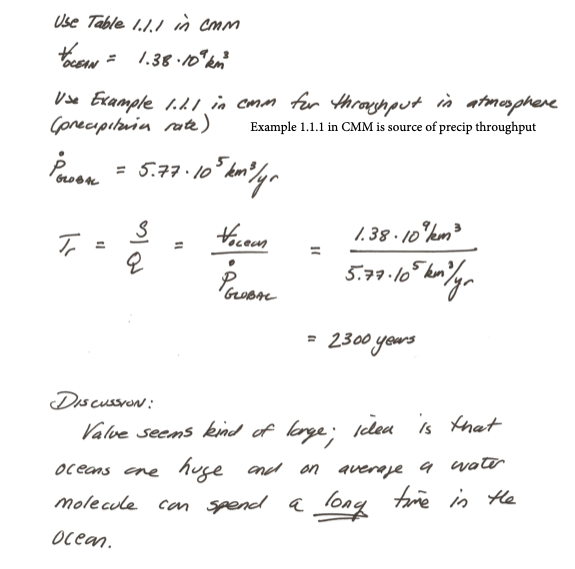
\includegraphics[width=6in]{es1-pr2-scan.png} 
   \caption{Ocean Residence Time Estimate}
   \label{fig:ocean_time}
\end{figure}

\clearpage
\item Assuming that all surface runoff to the oceans comes from rivers, estimate the average residence time of water in rivers. [Problem 1.1.2 in Chow, Maidment, and Mays]

\textbf{Solution(s)}

Figure \ref{fig:river_time} shows the estimated residence time of an arbitrary water molecule in the ocean using Table 1.1.1, and Table 1.1.2 in Chow, Maidment, and Mays.

\begin{figure}[h!] %  figure placement: here, top, bottom, or page
   \centering
   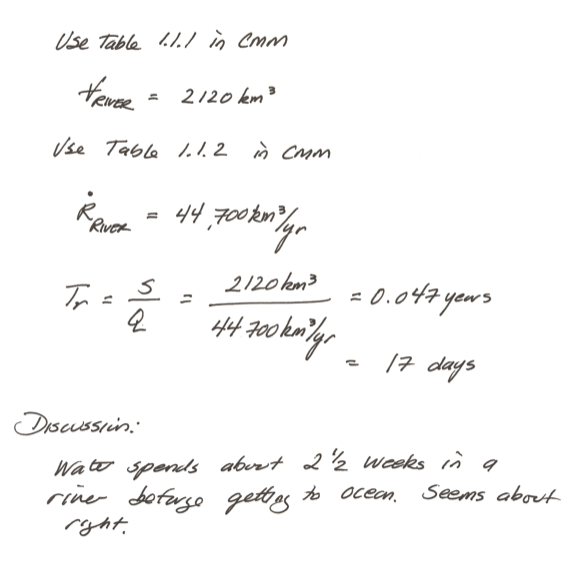
\includegraphics[width=6in]{es1-pr3-scan.png} 
   \caption{River Residence Time Estimate}
   \label{fig:river_time}
\end{figure}

\clearpage

\item The equation $k\frac{dQ}{dt} + Q(t) = I(t)$ has been used to describe the response of streamflow to a constant rate of precipitation continuing indefinitely on a watershed.  For this problem, let $I(t) =1$ for $t>0$ and $Q(t) =0$ for $t=0$. Plot values of $I(t)$ and $Q(t)$ over a 10-hour period if $k=2$.  [Problem 1.3.2 in in Chow, Maidment, and Mays]\footnote{You will need to solve the differential equation}

\textbf{Solution(s)}

Figure \ref{fig:es1-pr4-scan1} shows the analysis steps to produce an equation for plotting.

\begin{figure}[h!] %  figure placement: here, top, bottom, or page
   \centering
   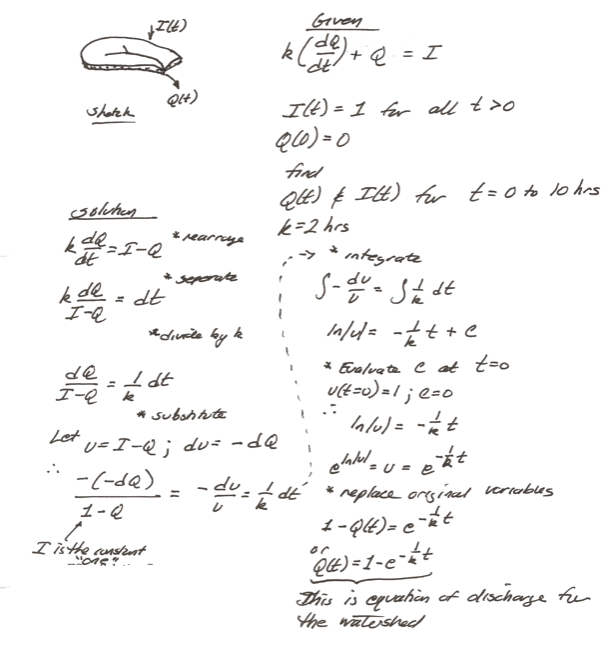
\includegraphics[width=5.5in]{es1-pr4-scan1.png} 
   \caption{Analysis to produce $Q=f(I,T)$ equation.}
   \label{fig:es1-pr4-scan1}
\end{figure}

\clearpage

Figure \ref{fig:es1-pr4-scan2} shows a script to plot of the resulting relationship.

\begin{figure}[h!] %  figure placement: here, top, bottom, or page
   \centering
   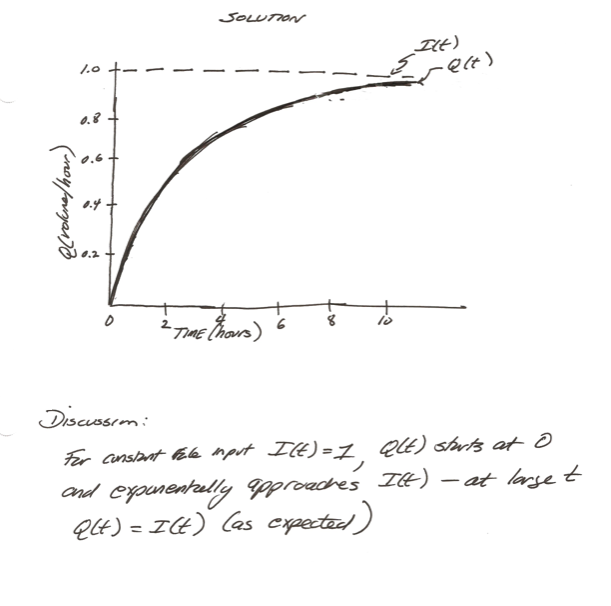
\includegraphics[width=6in]{es1-pr4-scan2.png} 
   \caption{Plot values of $I(t)$ and $Q(t)$ over a 10-hour period if $k=2$.}
   \label{fig:es1-pr4-scan2}
\end{figure}

\textbf{Chat GPT Solution}

Figures \ref{fig:chatgpt1of4} through \ref{fig:chatgpt4of4} show how to use a large-language model to assist in the solution to the ODE.  Note how the prompt is stated.  In this case the GPT solution is correct for the problem.

\begin{figure}[h!] %  figure placement: here, top, bottom, or page
   \centering
   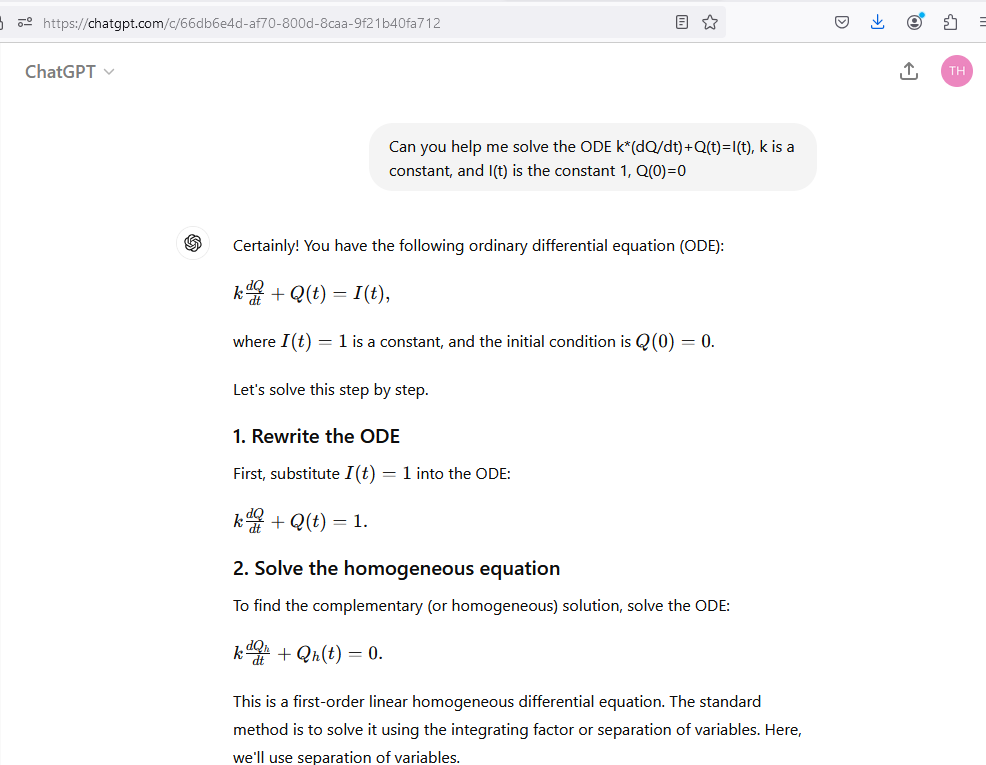
\includegraphics[width=6in]{chatgpt1of4.png} 
   \caption{Chat GPT ODE solution (1 of 4)}
   \label{fig:chatgpt1of4}
\end{figure}

\begin{figure}[h!] %  figure placement: here, top, bottom, or page
   \centering
   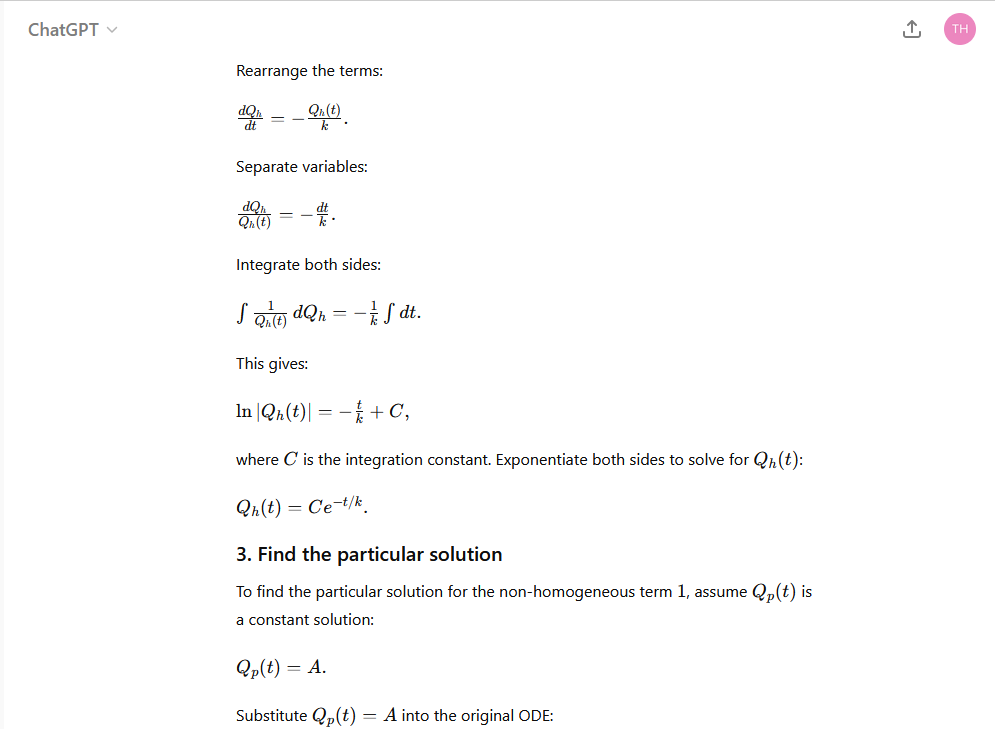
\includegraphics[width=6in]{chatgpt2of4.png} 
   \caption{Chat GPT ODE solution (2 of 4)}
   \label{fig:chatgpt2of4}
\end{figure}

\begin{figure}[h!] %  figure placement: here, top, bottom, or page
   \centering
   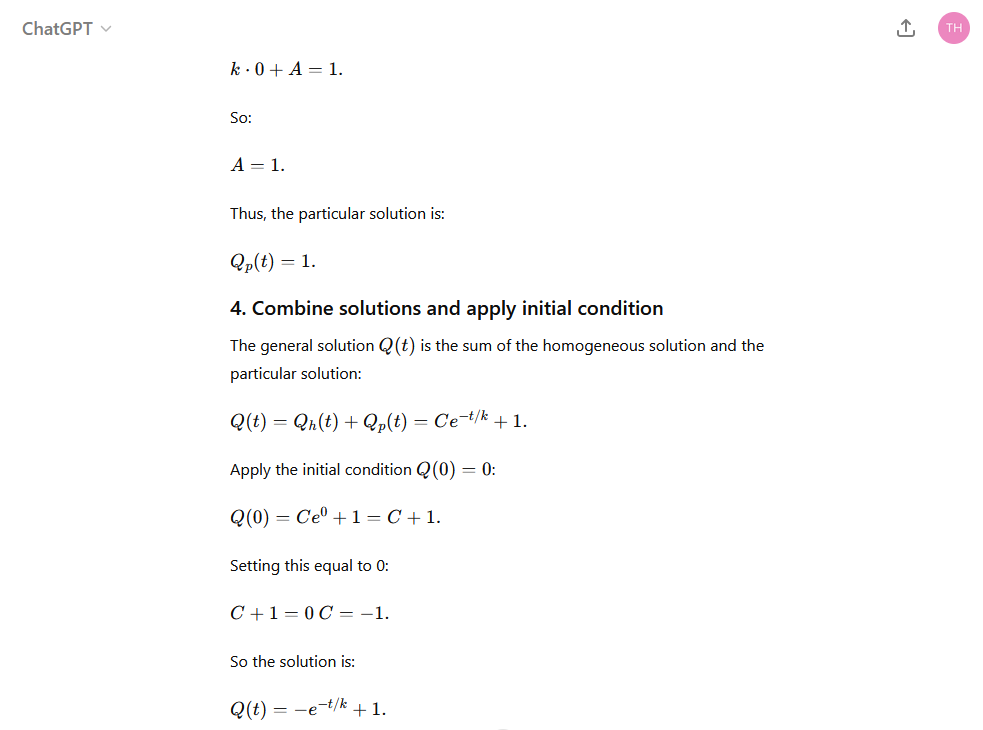
\includegraphics[width=6in]{chatgpt3of4.png} 
   \caption{Chat GPT ODE solution (3 of 4)}
   \label{fig:chatgpt3of4}
\end{figure}

\begin{figure}[h!] %  figure placement: here, top, bottom, or page
   \centering
   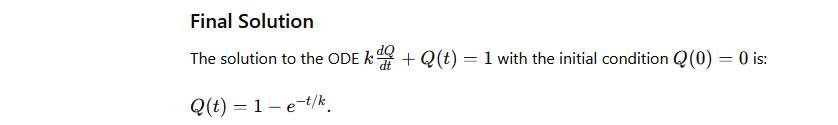
\includegraphics[width=6in]{chatgpt4of4.png} 
   \caption{Chat GPT ODE solution (4 of 4)}
   \label{fig:chatgpt4of4}
\end{figure}

\begin{figure}[h!] %  figure placement: here, top, bottom, or page
   \centering
   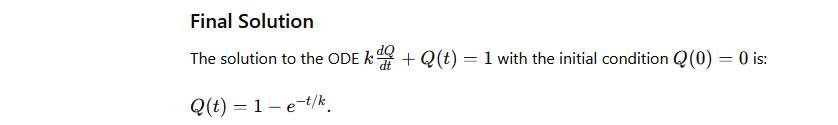
\includegraphics[width=6in]{chatgpt4of4.png} 
   \caption{Chat GPT ODE solution (4 of 4)}
   \label{fig:chatgpt4of4}
\end{figure}

\clearpage

Figure \ref{fig:es1-pr4-jupyter} shows a script to plot of the resulting relationship.

\begin{figure}[h!] %  figure placement: here, top, bottom, or page
   \centering
   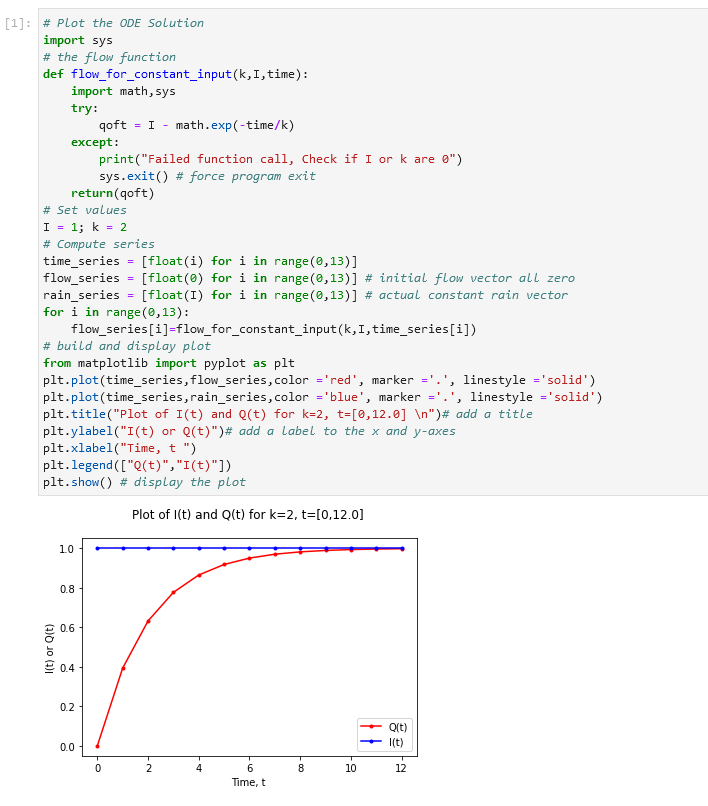
\includegraphics[width=6in]{es1-pr4-jupyter.png} 
   \caption{Plot values of $I(t)$ and $Q(t)$ over a 12-hour period if $k=2$.}
   \label{fig:es1-pr4-jupyter}
\end{figure}
 
\clearpage

%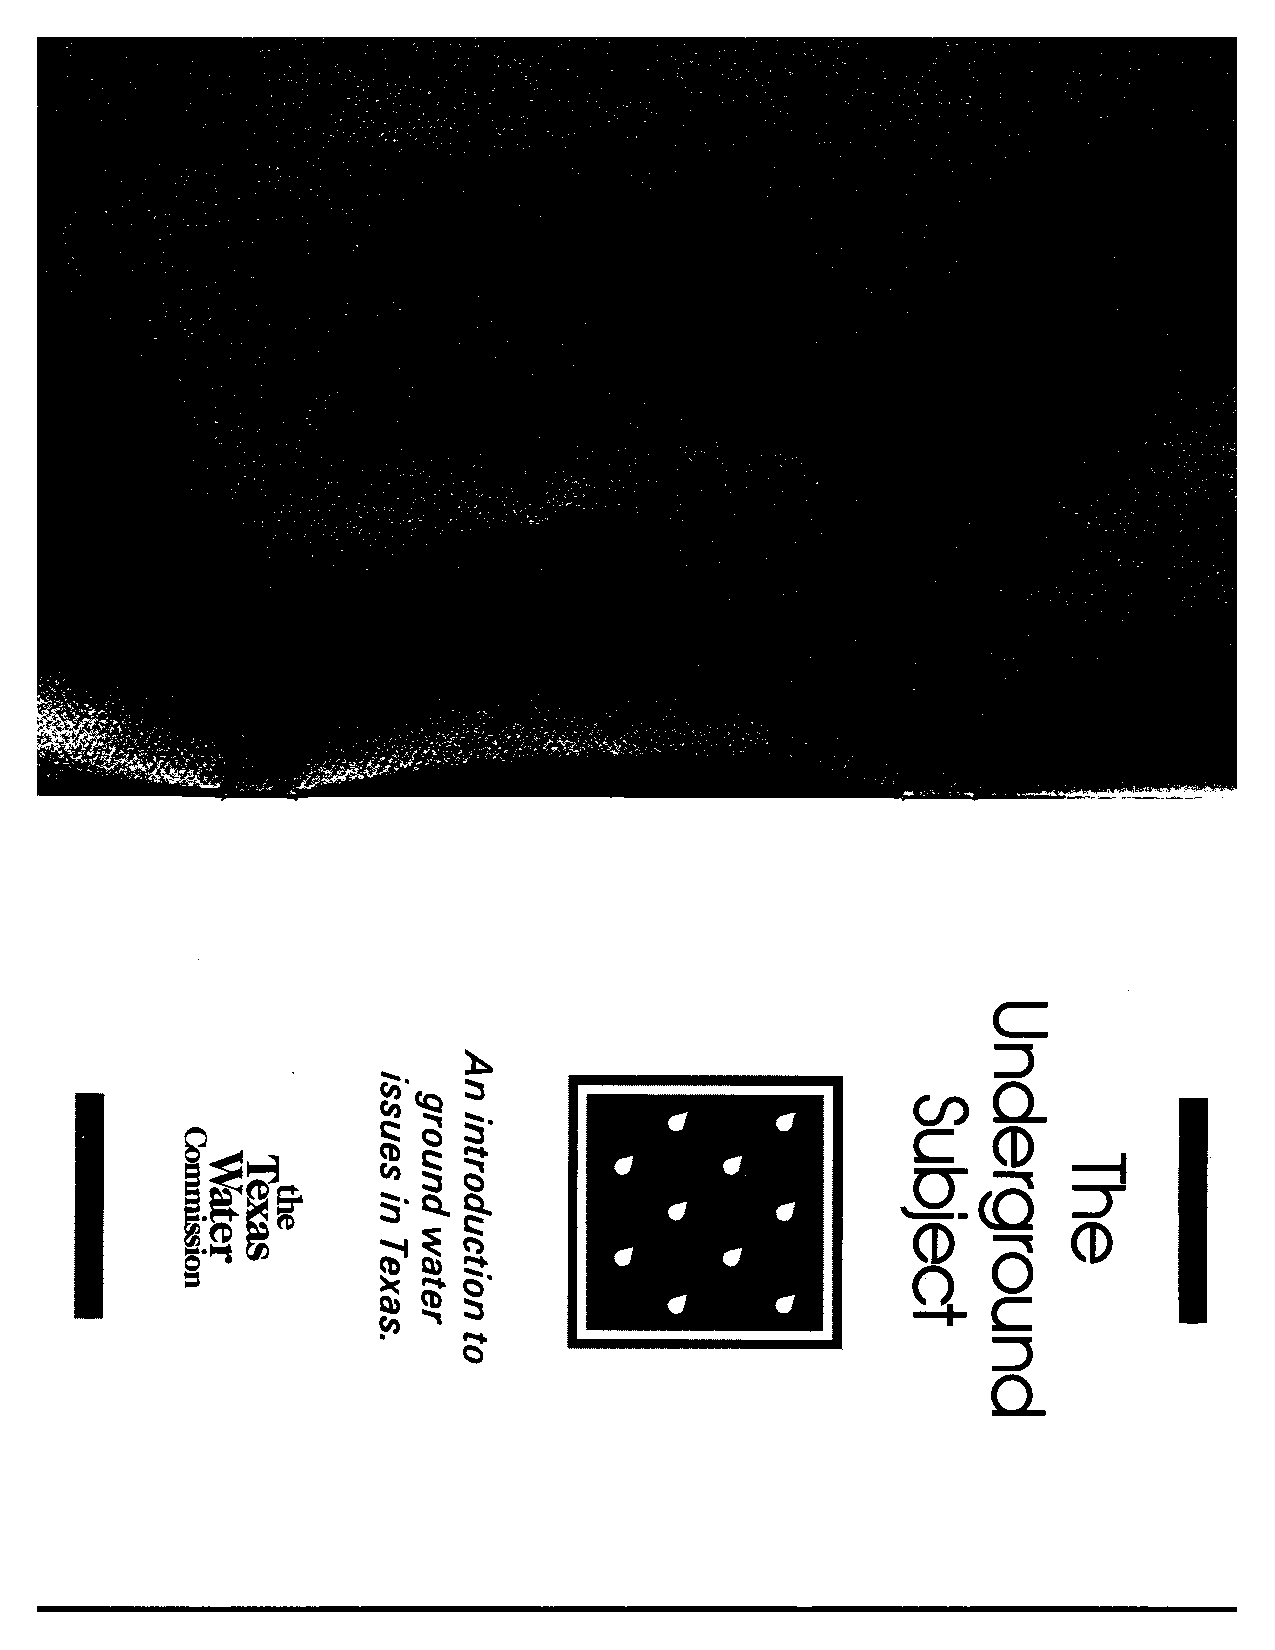
\includepdf[pages={-}]{./TWC_8905.pdf}
 
\item Figure \ref{fig:farmland} is a schematic of a 600-hectare farm; the land receives annual rainfall of 2500 mm.  There is a river flowing through the farm land with inflow rate of 5 m$^3$/s and outflow rate of 4m$^3$/s.  The annual water storage in the farm land increases by 2.5$\times$10$^6$m$^3$.  Using the water budget concept, estimate the annual evaporation amount in millimeters.\footnote{1 hectare = 10,000 m$^2$}

\begin{figure}[h!] %  figure placement: here, top, bottom, or page
   \centering
   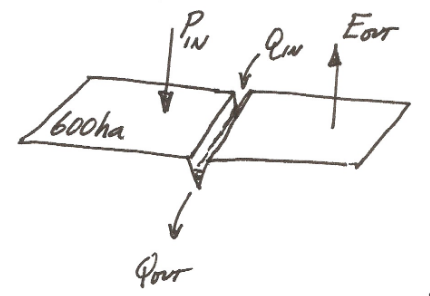
\includegraphics[width=4in]{farmland.png} 
   \caption{Schematic of Farmland}
   \label{fig:farmland}
\end{figure}

\textbf{Solution(s)}

Figure \ref{fig:river_farm} shows the estimated annual evaporation for the 600-hectare farm in \ref{fig:farmland}

\begin{figure}[h!] %  figure placement: here, top, bottom, or page
   \centering
   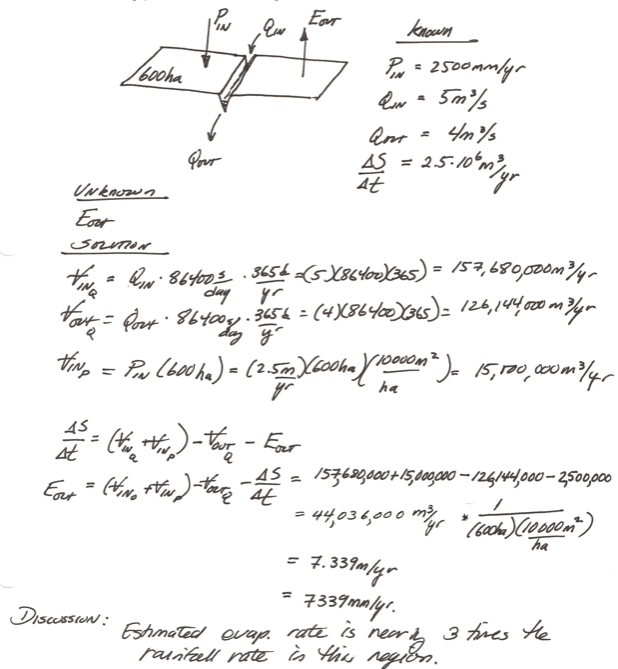
\includegraphics[width=6in]{es2-pr1-scan.png} 
   \caption{Farmland water balance estimates}
   \label{fig:river_farm}
\end{figure}

\clearpage

\item A reservoir has a surface area of 690 acres.  Figure \ref{fig:reservoir} shows the monthly inflow of surface water, outflows as releases from the reservoir via the spillway, direct precipitation into the reservoir, and evaporation from the reservoir.  The reservoir water surface elevation was 701.0 feet on January 1.  Determine the reservoir water surface elevation at the end of each month (i.e. complete the table)

\begin{figure}[h!] %  figure placement: here, top, bottom, or page
   \centering
   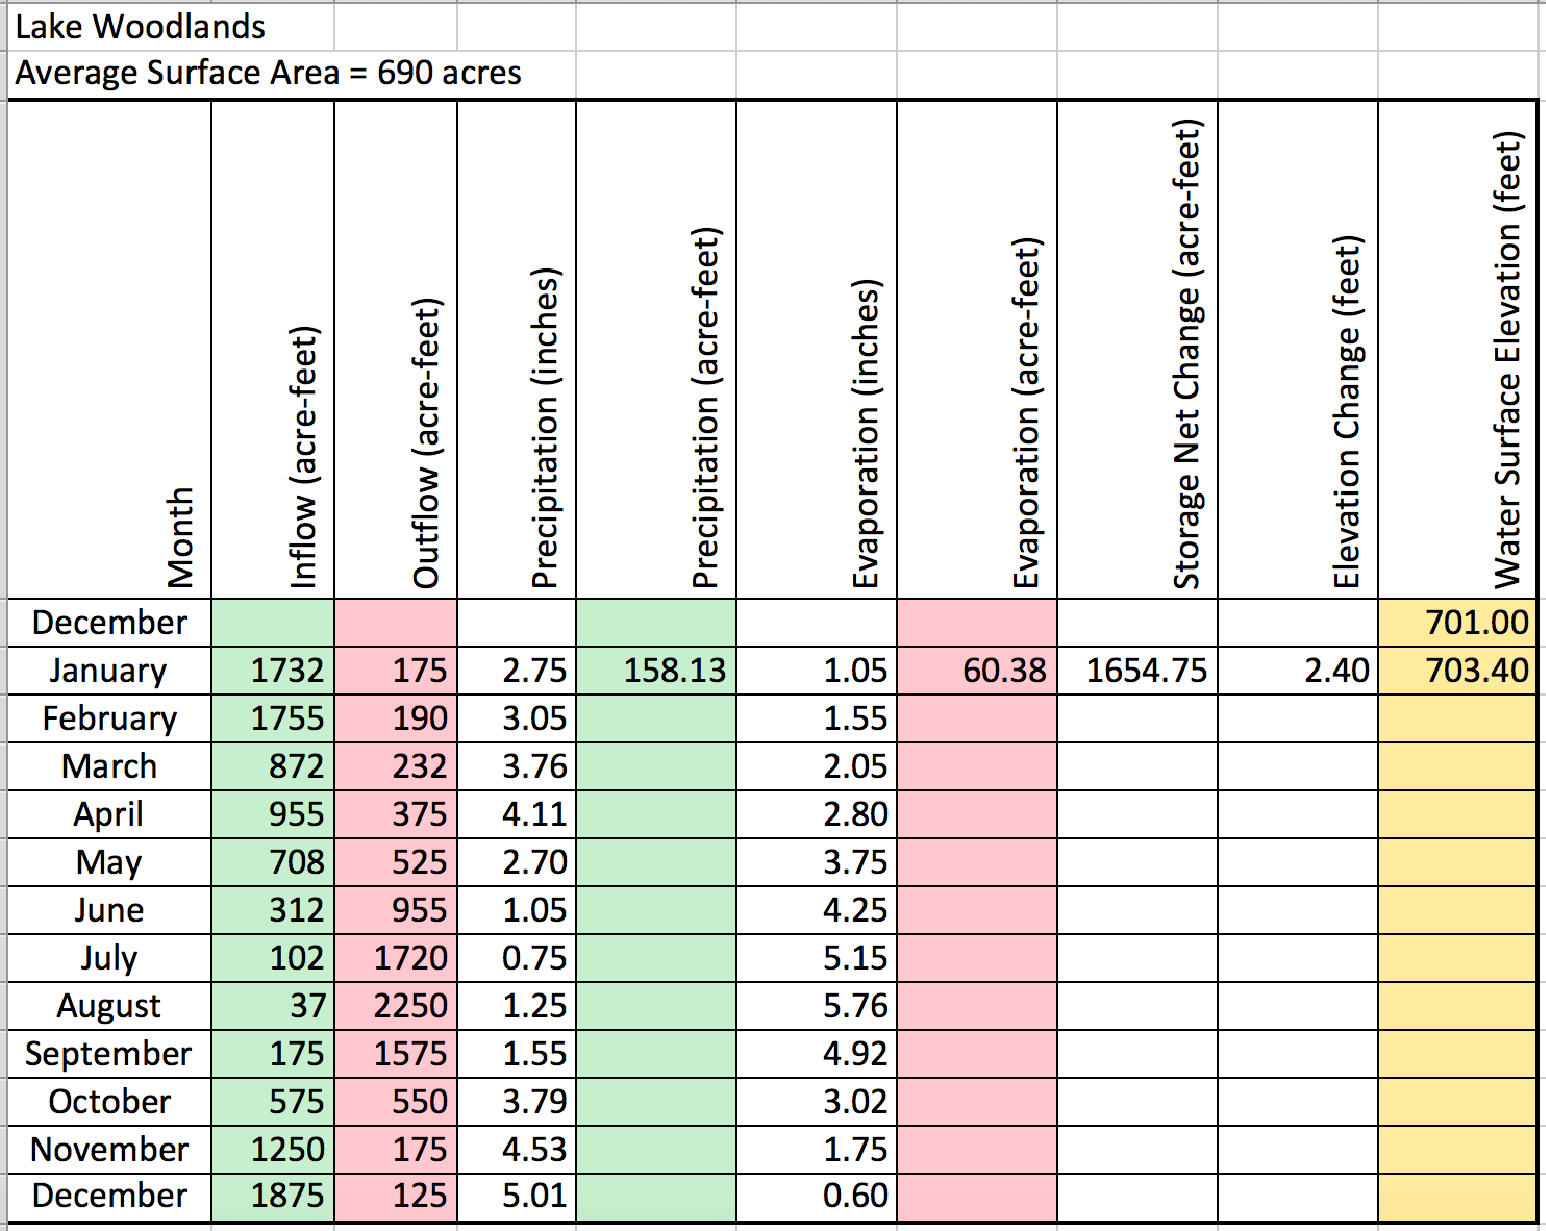
\includegraphics[width=6in]{Reservior.pdf} 
   \caption{Tabular Water Budget Values}
   \label{fig:reservoir}
\end{figure}

\textbf{Solution(s)}

Figure \ref{fig:es2-pr2-scan} shows the estimated water budget for the 690-acre reservoir.

\begin{figure}[h!] %  figure placement: here, top, bottom, or page
   \centering
   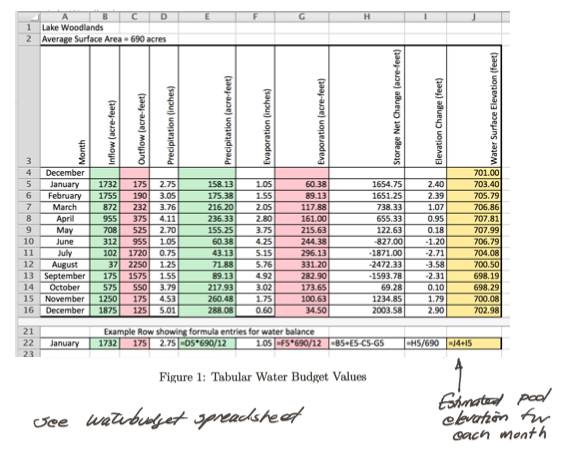
\includegraphics[width=6in]{es2-pr2-scan.png} 
   \caption{Tabular Water Budget (Complete - with annotations)}
   \label{fig:es2-pr2-scan}
\end{figure}

\end{enumerate}


\end{document}  

